\documentclass[conference]{IEEEtran}
\usepackage{graphicx}
\usepackage{cite}
\usepackage{url}
\usepackage[cmex10]{amsmath}
\usepackage{algorithmic}
\usepackage{array}
\usepackage{mdwmath}
\usepackage{mdwtab}
\usepackage{eqparbox}
\usepackage[font=footnotesize]{subfig}
\usepackage{fixltx2e}
\usepackage{setspace}
\usepackage{amssymb}

\begin{document}
\onehalfspacing
\title{A Reinforcement Learning Approach to Constrained Resource Allocation Problems}

\author{\IEEEauthorblockN{C. Vic Hu}
\IEEEauthorblockA{Department of Electrical \& Computer Engineering\\University of Texas at Austin}
}
\maketitle

\begin{abstract}
Resource allocation has been extensively studied in various fields such as wireless communication, intelligent traffic routing, industrial management, parallel architectures and distributed systems. Although there have been many efficient and powerful algorithms proposed in each domains, very few of them is able to address more generalized resource allocation problems on a higher level.
	
This paper proposes a generalized framework and makes three main contributions to solving constrained resource allocation problem using a modified reinforcement learning algorithm. First, we designed a general architecture, Constrained Resource Allocation Framework (CRAF), for the ease of generalized problem mapping and learning. Second, we defined four properties and three measurements to both quantitatively and qualitatively analyze how well an algorithm performs in CRAF. Finally, we developed three benchmark experiments to demonstrate how a reinforcement algorithm can successfully solve very different resource allocating problems with CRAF.
\end{abstract}

%Motivate and abstractly describe the problem you are addressing and how you are addressing it. What is the problem? Why is it important? What is your basic approach? A short discussion of how it fits into related work in the area is also desirable. Summarize the basic results and conclusions that you will present. 
\section{Introduction}
Resource allocation is an old and widely-solved problem in many fields, including electrical engineering, computer science, economics, management science and many more. It typically involves a fixed number of resource units to be distributed to a set of tasks over a period of time, such as landing aircraft scheduling, wireless communication routing, social security welfare and shared resources in parallel computer architectures. The problems of resource allocating are ubiquitous, but they all essentially boil down to one simple notion--based on a set of criteria, how many resource units should be allocated to which task first, and for how long.

To name a few remarkable research examples to solve this type of problems, Dresner and Stone proposed s reservation system for autonomous intersection management \cite{dresner2008} to allocate right of road for crossing traffic, Perkins and Royer presented a novel routing algorithm for ad-hoc on-demand mobile nodes management \cite{perkins1999}, and Foster et al. came up with a reservation and allocation architecture for heterogeneous resource management in computer network. While they all addressed an elegant solution to a specific domain, most of the techniques cannot be easily transferred to similar decision problems in other domains. In this paper, we focus on addressing exactly this issue and forming a general resource allocation framework that is suitable to be solved by a reinforcement learning method.

The first contribution of this paper is to form the Constrained Resource Allocation Framework (CRAF), in which we designed a generalized architecture to capture most of the resource allocation problems. In addition to the conventional first-come, first-served basis, we introduced the notion of constraints and queue propagation to reflect a more realistic setting and to relax more complicated systems into a single-frontier problem.

Secondly, we defined a collection of analysis criteria and evaluation methods to both qualitatively and quantitatively study how a reinforcement learning algorithm perform on our framework. Lastly, we proposed three benchmark problems to empirically demonstrate how CRAF applies to different resource allocation problems consistently and effectively.


\section{Background}

Unlike the Markov Decision Processes (MDPs) that most of the reinforcement learning algorithms are designed to solve, the notion of state representation, transition functions and reward functions in resource allocation problems such as aircraft landing scheduling can be very complex and challenging to define. Furthermore, the state space representing the entire global snapshot could be too large to be useful for effective learning. 

Instead of trying to model a resource allocation problem as MDP, we found it more intuitive to formalize it as a multi-armed bandit problem, which has been extensively researched in the field of reinforcement learning \cite{auer2002}. Assuming that we can reasonably classify each incoming task candidate to one of the K prototypes, from which we use the approximated reward functions to determine which candidate receives the resource unit in each episode. Before we formalize our definitions and notations of the framework, let us go through some of the existing K-armed algorithms and see how they can be useful to the resource allocation problem.

\subsection{The K-armed Bandit Problem}
The problem is formalized by a fixed number of slot gambling machines, each defined by a random variable $X_{i,n}$, for $1\leq i \leq K$ and $n \geq 1$. A sequential $N$ plays of machine $i$ give rewards of $X_{i,1},\,X_{i,2},\dots,\, X_{i,N}$, which are all independent of each other and identically distributed. Based on the sequence of playing history and obtained rewards, one can form an allocation algorithm to pick the next machine. To evaluate the performance of such algorithms, one criterion, the $regret$, is defined as

\begin{equation*}
	regret = \mu^{*}\,n - \mu_j \sum_{j=1}^K E[T_j(n)]
\end{equation*}

\noindent where $\mu_i$ is the true mean of the generative distribution of $X_i$, and $\mu^{*} \equiv \max_{1\leq i \leq K} \mu_i$, $T_j(n)$ is the number of times machine $j$ has been played during the n plays. Therefore, $regret$ is essentially the expected loss function (opportunity cost) of the played allocation strategy. In reality we don't know the true $\mu_i$ of any slot machines, and thus we need a more empirical method to estimate the payoffs. However, $regret$ gives us an intuition about one of the fundamental problem the reinforcement learning is trying to solve--the dilemma between exploration and exploitation.

\subsection{Balancing Exploration and Exploitation}
As introduced in the previous section, $regret$ is a theoretical index to tell us how close we are from the optimal playing strategy in a K-armed bandit game. To play the optimal action of the game, the learning agent needs to build up a knowledge base of how well each action will pay off. The behavior of trying unknown or low confident actions is called \emph{exploration}. At certain point, the agent may decide it is confident enough to simply play the best action based on the learned knowledge so far, and that playing a suboptimal \emph{exploration} policy is not worthwhile. This idea of greedily choosing whatever is currently the best is known as \emph{exploitation}. It is crucial that a learning agent need to balance both \emph{exploration} and \emph{exploitation} to find the optimal policy in almost any reinforcement learning settings. 

To quantitatively describe how `good' an action is, we can define the action-value function prior to time step $t$ to be
\begin{equation*}
	Q_t(a) = \frac{\sum_{i=1}^{N_a}r_i}{N_a}
\end{equation*}
\noindent where $N_a$ is the number of times action $a$ was chosen prior to $t$. In other words, $Q_t(a)$ is the sampled arithmetic average of the rewards received so far, which approaches to the true action-value $Q^{*}(a)$ as $N_a \rightarrow \infty$. Alternatively, instead of keeping track of the entire history of rewards received $r_i,\, i \in \{1,\dots,N_a\}$ we can simply increment the current action-value toward the new one with a step-size parameter $\alpha$:
\begin{equation*}
	Q_{k+1} = Q_k + \alpha\,[r_{k+1} - Q_k]
\end{equation*}
When we choose $\alpha = \frac{1}{k+1}$, the action-value function falls back to:
\begin{equation*}
	Q_{k+1} = \frac{1}{k+1} \sum_{i=1}^{k+1}r_i
\end{equation*}
\noindent Which is exactly the original sampled average form. To guarantee a  general step-size $\alpha$ such that $\lim_{k\rightarrow \infty}Q_k = Q^*$, it follows that the steps must be large enough to encounter biased initial conditions and randomness, while it cannot be too large for the action-value function to converge eventually. Based on these intuitions, the following conditions must hold according to the stochastic approximation theory in \cite{bertsekas1996}:
\begin{equation*}
	\sum_{k=1}^\infty \alpha_k(a) = \infty \text{ and } \sum_{k=1}^\infty \alpha_k^2(a) < \infty
\end{equation*}

One straightforward policy is to always exploit the greedy action $a^* = \arg\max_{a} Q_t(a)$to maximize the immediate reward at time $t$ . To balance \emph{exploitation} with \emph{exploration}, here are a few alternative methods we will consider:


\-\\
\textbf{$\epsilon$-greedy}: The simplest way is to explore once in a while and to exploit greedy actions the rest of the time. In other words, we can formalize a policy function as the probability of playing action $a$ at time $t$:
\begin{equation*}
	\pi_t(a) = 
	\begin{cases}
		1-\epsilon, & \text{for }a=a^* = \arg\max_{a} Q_t(a)\\
		\epsilon, & \text{choose any action randomly}
	\end{cases}
\end{equation*}

Although $\epsilon$-greedy method does guarantee $N_a \rightarrow \infty$ as $t \rightarrow \infty$ and thus $Q_t(a) \rightarrow Q^*(a)$ in theory, it is definitely not the most efficient learning strategy in practice, especially the evaluative feedback is non-stationary , which is true in most decision learning processes. However, it is a popular and effective way to balance exploration and exploitation when augmented with more sophisticated algorithms.

\-\\
\textbf{Softmax}: When exploring suboptimal actions, it makes more sense to choose risky action-values with lower probability, which intuitively blends in a little bit exploitation within the exploration itself. For instance, one may define the policy to be a probabilistic distribution in proportion to the action-values:
\begin{equation*}
	\pi_t(a) = \frac{e^{Q_t(a)/\tau}}{\sum_{\hat{a} \in A}e^{Q_t(\hat{a})/\tau}},\; \tau > 0
\end{equation*}

Notice that as the tuning parameter $\tau \rightarrow 0$, this softmax method is equivalent to the greedy policy, while higher $\tau$ leads to a more uniform action selection.


\-\\
\textbf{Reinforcement Comparison}: This method is based on a simple idea of ``preferring the good while avoiding the bad.'' Trivial and obvious as it sounds, we need to formalize our definitions of `preference' and `good/bad' to make this concept useful on a multi-armed bandit problem. First, we define the notion of the \emph{reference reward} at time $t$, $\overline{r}_t$:
\begin{equation*}
	\overline{r}_{t+1} = \overline{r}_t + \alpha\,[r_t - \overline{r}_t]
\end{equation*}
\noindent which is almost identical to the action-value function $Q_t$ we defined earlier, except that it is the incremental average of all the received rewards, regardless of the actions taken. Now we have the \emph{reference reward} to tell us what's the reward an average action should receive, we can establish our preference to an action based on its reward compared to the average:
\begin{equation*}
	p_{t+1}(a_t) = p_t(a_t) + \beta\,[r_t - \overline{r}_t],\, \beta > 0
\end{equation*}
\noindent which basically increases or decreases how much we prefer an action $a$ according to its reward, parameterized by another step-size parameter $\beta$. Finally, we can determine our policy just like the softmax method:

\begin{equation*}
	\pi_t(a) = \frac{e^{p_t(a)}}{\sum_{\hat{a} \in A}e^{p_t(\hat{a})}}
\end{equation*}

\-\\
\textbf{Pursuit}: The \emph{pursuit} method maintains both the action-value estimates $Q_t(a)$ for choosing the greedy action $a^*_t$ and the policy $\pi_t(a)$, which is updated by incrementing toward one and zero according to the following rule:
\begin{equation*}
	\pi_{t+1}(a) = 
	\begin{cases}
		\pi_{t}(a) + \beta\,\left[1-\pi_{t}(a)\right],& \text{for } a = a^*_{t+1}\\
		\pi_{t}(a) + \beta\,\left[0-\pi_{t}(a)\right],& \text{for } a \neq a^*_{t+1}\\
	\end{cases}
\end{equation*}

\-\\
\textbf{More Advanced Algorithms}: More recently, Auer et al. proposed a new set of more sophisticated algorithms to solve the multi-armed bandit problem in finite time \cite{auer2002}. Here we list a few that we consider to implement on our framework. The details and analysis of these algorithms are beyond the scope of this paper, but we encourage the reader to refer to their original work \cite{auer2002}

\-\\
\textbf{UCB1}: deterministic policy\\
\emph{Initialization}: play each action once\\
\emph{For each iteration}: play action $a^*$
\begin{equation*}
	a^*_t = \arg\max_{a \in A} Q_t(a) + \sqrt{\frac{2\ln N}{N_a}}
\end{equation*}
\noindent where $Q_t(a)$ is computed as the sampled average reward, $N_a$ is the number of $a$ played so far, and $N$ is the total rounds played ($N = \sum_{a \in A} N_a$)

\-\\
\textbf{UCB2}: deterministic policy\\
\emph{Initialization}: Set $r_a = 0\;\forall a \in A$ and play each action once\\
\emph{For each iteration}: 
\begin{enumerate}
	\item Choose 
	\begin{equation*}
		a^* = \arg\max_{a \in A} Q_t(a) + \sqrt{\frac{(1 + \alpha)\ln(e N /\tau(r_a))}{2 \tau(r_a)}}
	\end{equation*}
	\begin{equation*}
		\tau(x) = \lceil(1+\alpha)^x\rceil,\;0<\alpha<1
	\end{equation*}
	\item Play action $a$ exactly $\tau(r_a + 1) - \tau(r_a)$ times
	\item $r_a \leftarrow r_a + 1$
	\item slowly decrease $\alpha$
\end{enumerate}

\-\\
\textbf{$\epsilon_n$-greedy}: randomized policy ($\epsilon$ needs to go to 0)\\
\emph{Initialization}: Define $\epsilon_n \in (0,1],\,n=1,2,\dots$
\begin{equation*}
	\epsilon_n = min\{1, \frac{cK}{d^2n}\},\; c > 0 \text{ and }0 < d < 1 
\end{equation*}
\emph{For $n=1,2,\cdots$}: 
\begin{enumerate}
	\item Let $a_n = \arg\max_{a\in A} Q_n(a)$
	\item Play with action selected according to policy:
	\begin{equation*}
		\pi_n(a) = 
		\begin{cases}
			1 - \epsilon_n, & \text{for } a_n\\
			\epsilon_n, & random
		\end{cases}
	\end{equation*}
\end{enumerate}


\-\\
\textbf{UCB1-NORMAL}: deterministic policy \\
\emph{For $n=1,2,\cdots$}: 
\begin{enumerate}
	\item If $n_a < \lceil8\log{n}\rceil \; \forall a \in A$, play $a$
	\item Otherwise, play
	\begin{equation*}
		a^{*}_n = \arg\max_{a \in A} Q_n(a) + \sqrt{16 \cdot \frac{q_a - n_a Q^2_n(a)}{n_a - 1} \cdot \frac{\ln(n-1)}{n_a}}
	\end{equation*}
	\noindent where $q_a$ is the sum of squared rewards from action $a$ so far.
	\item Update $Q_n(a)$ and $q_a$ with the obtained reward
\end{enumerate}


%
%\-\\
%\textbf{UCB1-TUNED}: deterministic policy\\
%\emph{Initialization}: play each action once\\
%\emph{For each iteration}: play action $a^*$
%\begin{equation*}
%	a^*_t = \arg\max_{a \in A} Q_t(a) + \sqrt{\frac{\ln N}{N_a}\min\{1/4,V_a(N_a)\}}
%\end{equation*}
%
%

\-\\



\subsection{Prototype Classification}


\subsubsection{Distance Functions}
The idea of a particle is essentially a sampled instance of the topic distribution over a time sequence, represented by a vector $\mathbf{w}_i\in \mathbb{R}^{|V|},\; i \in \{1,\cdots,N\}$, where $|V|$ is the total vocabulary size of all the topic words appeared. Since one of our intermediate objectives is to formalize clusters between these particles, we need to first define how we will measure the similarity or distance between any pair of particles $\mathbf{w}_i,\; \mathbf{w}_j$. 

\-\\
\textbf{Minkowski}: 
\begin{equation*}
	d = \sqrt[p]{\sum_{k=1}^{|V|}|w_{ik} - w_{jk}|^p}
\end{equation*}
 Note that when $p=1$, the Minkowski reduces to the city block distance, while $p=2$ gives the Euclidean distance and $p=\infty$ yields the Chebychev distance.

\-\\
\textbf{Cosine}: 
\begin{equation*}
d = 1 - \frac{\mathbf{w}_i\,\mathbf{w}_j^T}{|\mathbf{w}_i|_2|\mathbf{w}_j|_2}
\end{equation*}

\-\\
\textbf{Correlation}: 
\begin{equation*}
d = 1 - \frac{(\mathbf{w}_i - \overline{\mathbf{w}}_i)(\mathbf{w}_j - \overline{\mathbf{w}}_j)^T}{|(\mathbf{w}_i - \overline{\mathbf{w}}_i)|_2|(\mathbf{w}_j - \overline{\mathbf{w}}_j)|_2}
\end{equation*}

where 
\begin{equation*}
	\overline{\mathbf{w}}_i = \frac{1}{|V|}\sum_{k=1}^{|V|}w_{ik},\;
	\overline{\mathbf{w}}_j = \frac{1}{|V|}\sum_{k=1}^{|V|}w_{jk}
\end{equation*}

\-\\
\textbf{Jaccard}: 
\begin{equation*}
	d = \frac{\# \left[(w_{ik} \neq w_{jk})\cap((w_{ik} \neq 0)\cup(w_{jk} \neq 0))\right]}{\#\left[(w_{ik} \neq 0)\cup(w_{jk} \neq 0)\right]}
\end{equation*}

\-\\

\subsubsection{Clustering Algorithms}
LDA is essentially pulling out the `principal components' from the text documents, reducing a large archive of data into just $K$ representative topics $\mathbf{\beta}_{1:K}$. Therefore, our assumption is that by grouping similar particles induced from past topics, we can observe the clustering patterns and make reasonable predictions on how the future topics will be like.

Now we have a collection of well-defined distance functions, we can start looking at clustering methods to group our particles together accordingly, and here are a set of common clustering algorithms we will consider:

\-\\
\textbf{K-Means:} As the name itself suggests, the K-Means clustering algorithm consists of K cluster centroids and moves these means iteratively towards the center of its closest neighbors, until they no longer change. Although K-Means has been proved to be guaranteed for convergence \cite{selim1984}, its clustering performance is often correlated to how the seeds are initialized at the beginning, and the optimal choice of $K$ is often not apparent (in our case, it is the same as the number of topics.)

\begin{verbatim}
1. Initialize the means by picking 
   K samples at random
2. Iterate
2.a. Assign each instance to 
     its nearest mean
2.b. Move the current means to 
	 the center of all the 
	 associated points
\end{verbatim}
\-\\
\textbf{Hierarchical Agglomerative Clustering (HAC):} This algorithm starts with treating every instances as individual cluster, and iteratively joins pairs of similar clusters repeatedly until there is only one. If we take the merging history and form a hierarchical binary tree, it will look like the dendrogram in Fig.~\ref{dendrogram}.

\begin{figure}[h]
	\center	
	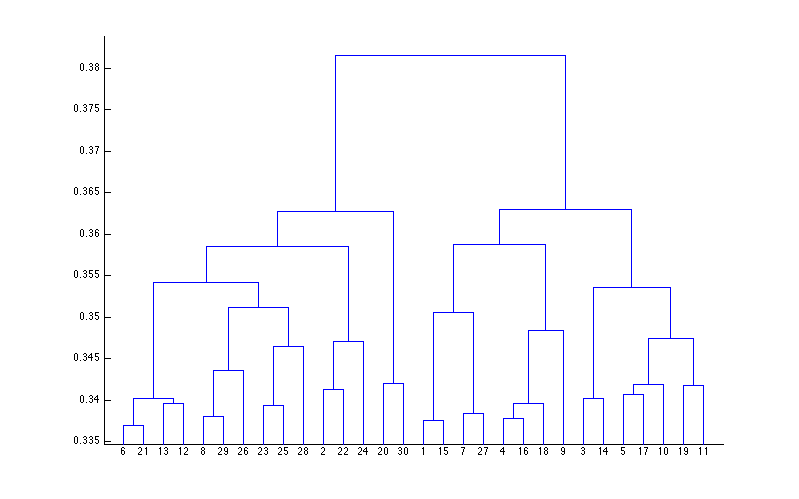
\includegraphics[width=0.35\textwidth]{fig/dendrogram.png}
	\caption{A sample dendrogram by HAC}
	\label{dendrogram}
\end{figure}

Although we have defined the distance functions in the previous section, we have yet formalized the similarity functions between clusters. In our method, we will focus on the following four similarity functions:

\begin{itemize}
	\item \textbf{Single-linkage:} Also known as the nearest neighbor, computes the distance between the two closest elements from two clusters
	\item \textbf{Complete-linkage:} The conjugate of \textbf{single-linkage}, also known as the farthest neighbor, computes the distance between the two farthest elements (maximum distance) from two clusters
	\item \textbf{UPGMA: } Unweighted Pair Group Method with Averaging calculates the distance between two clusters, $C_i \& C_j$, by averaging all distances between any pair of objects from the two clusters.
	\begin{equation*}
		dist(C_i, C_j) = \frac{1}{|C_i||C_j|}\sum_{w_i \in C_i}\sum_{w_j \in C_j}dist(w_i, w_j)
	\end{equation*}
	Now, let's call this newly-formed cluster $C_{ij}$ and compare its distance with another cluster $C_k$:
	\begin{equation*}
		dist(C_{ij}, C_k) =  \frac{|C_i|dist(c_i,c_k) + |C_j|dist(c_j,c_k)}{|C_i|+|C_j|}
	\end{equation*}
	where $c_i,\,c_j,\,c_k$ are the centroids for clusters $C_i,\;C_j,\;C_k$
	\item \textbf{WPGMA} Weighted Pair Group Method with Averaging is similar to UPGMA except that the cluster distance is now calculated as:
	\begin{equation*}
		dist(C_{ij}, C_k) =  \frac{dist(c_i,c_k) + dist(c_j,c_k)}{2}
	\end{equation*}
\end{itemize}

 The behavior of HAC is often dominated by the chosen similarity function. While each variant has a different set of clustering patterns it is good at capturing, all of them have certain vulnerabilities. 

%
%\subsection{The Adaptive K-Meteorologist Algorithm}
%One just moved to a new city with K TV news channels, what's the optimal strategy to determine the best meteorologist for weather prediction? Diuk et al.
%
%\subsection{Met-Rmax}
%
%\subsection{SCRAM-Rmax}
%
%\subsection{Gittins Index}
%
%\subsection{Thompson Sampling}

%Precisely define the problem you are addressing (i.e. formally specify the inputs and outputs). Elaborate on why this is an interesting and important problem. 

%Describe in reasonable detail the algorithm you are using to address this problem. A psuedocode description of the algorithm you are using is frequently useful. Trace through a concrete example, showing how your algorithm processes this example. The example should be complex enough to illustrate all of the important aspects of the problem but simple enough to be easily understood. If possible, an intuitively meaningful example is better than one with meaningless symbols. 
\section{The Constrained Resource Allocation Framework}

Formally, the Constrained Resource Allocation Framework (CRAF) consists of a sequential task instances, and a centralized learning agent who distributes resource units to the task instances and receives rewards according to the decision they make. The task instances can come in one or more channels $\mathbf{x}_{c,i},\, 1\leq c \leq C,\, 1\leq i \leq capacity(c)$, where $i$ denotes the i-th instance and $c$ denotes the c-th channel. To transform a resource allocation problem into a learnable framework, the formalization process under CRAF can be broke down into three phases:

\begin{enumerate}
	\item Housekeeping Phase
	\begin{itemize}
		\item \textbf{Constraint}: The instance $x_{c,i}$ needs a total of $num(x_{c,i})$ resource units before the deadline $exp(x_{c,i})$
		\item \textbf{Objective}: A high-level criteria that the learning agent should achieve, which adds bias against the reward functions
	\end{itemize}
	\item Tuning Phase
	\begin{itemize}
		\item \textbf{Priority Score}: $ps(x_{c,i})$, a function of both the \textbf{Constraint} and \textbf{Objective}
		\item \textbf{Queue Propagation}: $qp(x_{c,i}) = \gamma qp(x_{c,i+1}) + \tau \,ct(x_{c,i})$ A linear combination of the current constraint and the same function from the next instance in queue
		\item \textbf{Failure Capture}: If the current instance's constraint is impossible to be fulfilled or fails to respond, a \emph{reject} message will be sent and no further request from the same instance will be considered (so it will have to re-enter the queue)
	\end{itemize}
	\item Prototyping Phase
	\begin{itemize}
		\item \textbf{Prototype Classification}: Given a manually-chosen $K$, the current instance $x_{c,i}$ is classified into one of the $K$ clustering prototypes with respect to the two parameters obtained in the previous phase $ps(x_{c,i}),\, qp(x_{c,i})$
		\item \textbf{Reward Function}: The learning agent receives a reward of $r_p+r_o$ if it fulfills the constraint of $x_{c,i}$, or $r_f-r_o$ otherwise
	\end{itemize}
\end{enumerate}

Now we have formed the $K$ prototypes, we can have the resource allocating agent learn to choose from the channel frontiers just like in the multiarmed bandit problem.

\newpage

%
%Instance -> observables
%Constraints -> rewards
%Prototype
%Capacity -> resources available (treat each token as a multi-agent unit)
%Queue propagation (only solve the frontier instances at each round)
%
%failure handling
%
%
%properties:
%fairness
%progression
%safety
%liveness
%
%measurements:
%latency
%throughput
%rewards


%What are criteria you are using to evaluate your method? What specific hypotheses does your experiment test? Describe the experimental methodology that you used. What are the dependent and independent variables? What is the training/test data that was used, and why is it realistic or interesting? Exactly what performance data did you collect and how are you presenting and analyzing it? Comparisons to competing methods that address the same problem are particularly useful. 

%Present the quantitative results of your experiments. Graphical data presentation such as graphs and histograms are frequently better than tables. What are the basic differences revealed in the data. Are they statistically significant? 
\section{Experimental Results}
1. 2-way intersection (simplest form)
2. 4-way intersection (special corner cases)
3. n-children candy distribution (multi-channel)
%taxi sharing

%autonomous intersection management
%household welfare

%Answer the following questions for each piece of related work that addresses the same or a similar problem. What is their problem and method? How is your problem and method different? Why is your problem and method better? 
\section{Discussion and Related Work}



%Is your hypothesis supported? What conclusions do the results support about the strengths and weaknesses of your method compared to other methods? How can the results be explained in terms of the underlying properties of the algorithm and/or the data. 

%Briefly summarize the important results and conclusions presented in the paper. What are the most important points illustrated by your work? How will your results improve future research and applications in the area? 
\section{Conclusion}


%What are the major shortcomings of your current method? For each shortcoming, propose additions or enhancements that would help overcome it. 
\section{Future Work}


\section{Acknowledgements}

%Be sure to include a standard, well-formated, comprehensive bibliography with citations from the text referring to previously published papers in the scientific literature that you utilized or are related to your work.
\begin{thebibliography}{1}
\bibitem{dresner2008}
Dresner, K. and Stone, P. A Multiagent Approach to Autonomous Intersection Management. \begin{em}Journal of Artificial Intelligence Research\end{em}, 31:591-656, March 2008.

\bibitem{perkins1999}
Perkins, C. E., and Royer, E. M. (1999, February). Ad-hoc on-demand distance vector routing. In \begin{em}Mobile Computing Systems and Applications, 1999. Proceedings. WMCSA'99. Second IEEE Workshop on (pp. 90-100).\end{em} IEEE.

\bibitem{foster1999}
Foster, I., Kesselman, C., Lee, C., Lindell, B., Nahrstedt, K., and Roy, A. (1999). A distributed resource management architecture that supports advance reservations and co-allocation. In \begin{em}Quality of Service, 1999. IWQoS'99. 1999 Seventh International Workshop on (pp. 27-36).\end{em} IEEE.

\bibitem{baruah1996}
Baruah, S. K., Cohen, N. K., Plaxton, C. G., and Varvel, D. A. (1996). Proportionate progress: A notion of fairness in resource allocation. \begin{em}Algorithmica\end{em}, 15(6), 600-625.

\bibitem{thomas1990}
Thomas, D. (1990). Intra-household resource allocation: An inferential approach. \begin{em}Journal of human resources\end{em}, 635-664.

\bibitem{auer2002}
Auer, P., Cesa-Bianchi, N. and Fischer, P. Finite-time Analysis of the Multiarmed Bandit Problem. In \begin{em} Proc. of 15th International Conference on Machine Learning, pages 100-108\end{em}. Morgan Kaufmann, 1998.

\bibitem{diuk2009}
Diuk, C., Li, L. and Leffler, B. R. The Adaptive k-Meteorologists Problem and Its Application to Structure Learning and Feature Selection in Reinforcement Learning. In \begin{em} Proceedings of the 26th International Conference of Machine Learning\end{em}. Montreal, Canada, 2009. 

\bibitem{bertsekas1996}
Bertsekas, D. P., and Tsitsiklis, J. N. (1996). Neuro-Dynamic Programming (Optimization and Neural Computation Series, 3). \begin{em}Athena Scientific\end{em}, 7, 15-23.

\end{thebibliography}




% that's all folks
\end{document}


